\documentclass{beamer}

\mode<presentation>
{
    \usetheme{Madrid}         % or try Darmstadt, Madrid, Warsaw, ...
    \usecolortheme{default}   % or try albatross, beaver, crane, ...
    \usefonttheme{default}    % or try serif, structurebold, ...
    \setbeamertemplate{navigation symbols}{}
    \setbeamertemplate{caption}[numbered]
} 

\usepackage[UTF8]{ctex}
\usepackage{ulem}
\usepackage{enumerate}
\usepackage{amsmath,amsthm,amsfonts,amssymb,amscd}

\title[Algorithms and Exercises]{Algorithms and Exercises}
\author{YouSiki}
\institute{Peking University}
\date{2019.7.13-2019.7.14}

\begin{document}

\begin{frame}
    \titlepage
\end{frame}

\section{Introduction}

\begin{frame}{Introduction}

    \begin{itemize}
        \item 
        Algorithms
        \begin{enumerate}
            \item 搜索 search
            \item 贪心 greedy
            \item 二分 binary search
            \item 倍增 multiplication
            \item 分治 divide and conquer
            \item 其它 others
        \end{enumerate}
        \item
        Exercises
        
        习题来自各种在线测评平台
    \end{itemize}

\end{frame}

\section{Algorithms}

\subsection{Search}

\begin{frame}{搜索 Search}

    回归主流考点
    
    多多切题巩固
    
    \begin{enumerate}
        \item 
        迭代加深
        \item
        估价函数
        \item
        IDA*
    \end{enumerate}
    
\end{frame}

\begin{frame}{HDU 4127 Flood-it!}

    Flood-it is a fascinating puzzle game on Google+ platform.
    
    At the beginning of the game, system will randomly generate an N×N square board and each grid of the board is painted by one of the six colors. The player starts from the top left corner. At each step, he/she selects a color and changes all the grids connected with the top left corner to that specific color. The statement “two grids are connected” means that there is a path between the certain two grids under condition that each pair of adjacent grids on this path is in the same color and shares an edge. In this way the player can flood areas of the board from the starting grid (top left corner) until all of the grids are in same color. 
    
    Given a colored board at very beginning, please find the minimal number of steps to win the game (to change all the grids into a same color). 
    
\end{frame}

\begin{frame}{HDU 4127 Flood-it!}

    \begin{figure}
        \centering
        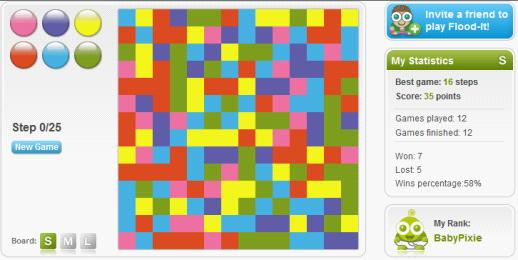
\includegraphics[width=0.5\textwidth]{hdu4127-1.jpg}
        \caption{game interface}
    \end{figure}
    
    \begin{figure}
        \centering
        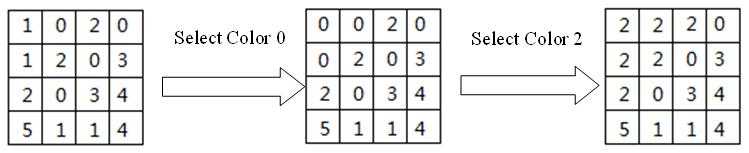
\includegraphics[width=0.9\textwidth]{hdu4127-2.jpg}
        \caption{the earliest steps of a 4×4 game}
    \end{figure}
    
\end{frame}

\begin{frame}{HDU 4127 Flood-it!}

    \begin{itemize}
        \item BFS:$8\times8\times6$状态数太大,难以保存
        \item DFS:朴素搜索难以在规定时间内通过
        \item IDA* DFS:估价函数、剪枝策略?
    \end{itemize}
    
\end{frame}

\begin{frame}{HDU 4127 Flood-it!}

    \begin{itemize}
        \item 估价函数
        
            记当前颜色种类数为$c$,则至少需要$c-1$步
        
        \item 剪枝策略
        \begin{itemize}
            \item 枚举的颜色不能为当前左上角颜色
            \item 枚举的颜色要令左上角连通块扩大
            \item 记录哪些点已经并入左上角连通块,而非每次暴力修改棋盘颜色
            \item ...
        \end{itemize}
    \end{itemize}
    
\end{frame}

\begin{frame}{HDU 2234 无题}

    一天机器人小A在玩一个简单的智力游戏,这个游戏是这样的,在一个4*4的矩阵中分别有4个1,4个2,4个3和4个4分别表示4种不同的东西,每一步小A可以把同一行的4个数往左移或者往右移一步或者把同一列的4个数字往上移或者往下移一步(1,2,3,4往左移后是2,3,4,1),小A现在想知道进过最少的几步移动可以将矩阵的每行上的4个数字都一样或者每列上的4个数字都一样。但是小A又不想走太多步,他只要知道最少步数是否少于等于5步,是的话输出准确的步数,否则输出-1。
    
\end{frame}

\begin{frame}{HDU 2234 无题}

    \begin{itemize}
        \item 和POJ的The Rotation Game非常相似
        \item IDA*
        \item 估价函数
        
            假设以最终每行数字均相同为目标。
            记第$i$行众数的出现次数为$a_i$,
            则至少需要改变该行内$4-a_i$个数字。
            行变换不改变行内数字,
            列变换一次最多改变$4$个行内数字。
            所以最少需要$\lceil\frac{\sum_{i=1}^4{4-a_i}}{4}\rceil$步。
            记第$i$列众数的出现次数为$b_i$,
            最终估价函数即为
            $$min\{\lceil\frac{\sum_{i=1}^4{4-a_i}}{4}\rceil,\lceil\frac{\sum_{i=1}^4{4-b_i}}{4}\rceil\}$$
        \end{itemize}
    
\end{frame}

\begin{frame}{HDU 2918 Tobo or not Tobo}

    The game of Tobo is played on a plastic board designed into a 3 × 3 grid with cells numbered from 1 to 9 as shown in figure (a). The grid has four dials (labeled ``A" to ``D" in the figure.) Each dial can be rotated in 90 degrees increment in either direction. Rotating a dial causes the four cells currently adjacent to it to rotate along. For example, figure (b) shows the Tobo after rotating dial ``A" once in a clockwise direction. Figure (c) shows the Tobo in figure (b) after rotating dial ``D" once in a counterclockwise direction. 
    
    \begin{figure}
        \centering
        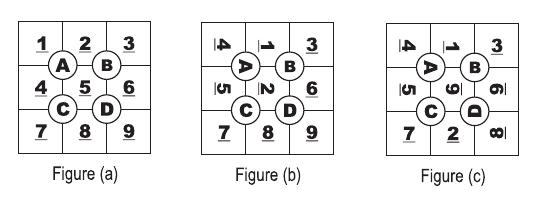
\includegraphics[width=0.9\textwidth]{hdu2918.jpeg}
    \end{figure}
    
\end{frame}
    
\begin{frame}{HDU 2918 Tobo or not Tobo}

    Kids love to challenge each other playing the Tobo. Starting with the arrangement shown in figure (a), (which we'll call the standard arrangement,) one kid would randomly rotate the dials, X number of times, in order to ``shuffle" the board. Another kid then tries to bring the board back to its standard arrangement, taking no more than X rotations to do so. The less rotations are needed to restore it, the better. This is where you see a business opportunity. You would like to sell these kids a program to advise them on the minimum number of steps needed to bring a Tobo back to its standard arrangement.
    
    Your program will be tested on one or more test cases. Each test case is specified on a line by itself. Each line is made of 10 decimal digits. Let's call the first digit Y . The remaining 9 digits are non-zeros and describe the current arrangement of the Tobo in a row-major top-down, left-to-right ordering. If it can't be done in Y dials or less, then the answer should be -1.
    
\end{frame}

\begin{frame}{HDU 2918 Tobo or not Tobo}
    
    \begin{itemize}
        \item BFS:$9!=362880$状态太大
        \item DFS:IDA* 如何设计估价函数
    \end{itemize}
    
\end{frame}

\begin{frame}{HDU 2918 Tobo or not Tobo}
    
    \begin{itemize}
        \item 定义错误:数字$x_i$不在目标位置上,记为一个错误
        \item 每次旋转,最多使错误减少4
        \item 估价函数:$\lceil\frac{TotalError}{4}\rceil$
    \end{itemize}
    
\end{frame}

\begin{frame}{HDU 2918 Tobo or not Tobo}
    
    \begin{itemize}
        \item 定义距离:数字$x_i$到目标位置的曼哈顿距离
        \item 每次旋转,最多使总距离减少4
        \item 估价函数:$\lceil\frac{TotalDistance}{4}\rceil$
    \end{itemize}
    
\end{frame}

\begin{frame}{HDU 1813 Escape from Tetris}

    由于整日整夜地对着这个棋盘,Lele终于走火入魔。每天一睡觉,他就会梦到自己会被人被扔进一个棋盘中,一直找不到出路,然后从梦中惊醒。久而久之,Lele被搞得精神衰弱。梦境是否会成为现实,谁也说不准,不过不怕一万只怕万一。现在Lele每次看到一个棋盘,都会想象一下自己被关进去以后要如何逃生。
    
    Lele碰到的棋盘都是正方形的,其中有些格子是坏的,不可以走,剩下的都是可以走的。只要一走到棋盘的边沿(最外面的一圈),就算已经逃脱了。Lele梦见自己一定会被扔在一个可以走的格子里,但是不确定具体是哪一个,所以他要做好被扔在任意一个格子的准备。
    
    现在Lele请你帮忙,对于任意一个棋盘,找出一个最短的序列,序列里可以包括"north"(地图里向上),"east"(地图里向右),"south"(地图里向下),"west"(地图里向左),这四个方向命令。不论Lele被扔在棋盘里的哪个好的格子里,都能按这个序列行走逃出棋盘。
    逃脱的具体方法是:不论Lele被扔在哪里,Lele按照序列里的方向命令一个一个地走,每个命令走一格,如果走的时候会碰到坏的格子,则忽略这条命令。当然,如果已经逃脱了,就可以不考虑序列中剩下的命令了。$0<N<9$
    
\end{frame}

\begin{frame}{HDU 1813 Escape from Tetris}

    \begin{itemize}
        \item 目标:满足要求的最短的、字典序最小的NESW序列
        \item 
        搜索过程中依次枚举第$i$位,
        可以视为若干小人从各个空格子出发,
        按照指定的方向序列行走,
        最终让所有小人都走到边界。
        \item 
        不论向哪个方向行走,每个小人最多离边界更近一步。
        记第$j$个小人当前距离边界的最近距离为$d_j$,
        则需要至少$max\{d_j\}$步。
        \item 
        为了保证字典序最小,枚举顺序应为ENSW。
    \end{itemize}
    
\end{frame}

\subsection{Greedy}

\begin{frame}{贪心 Greedy}

    \begin{itemize}
        \item 寻找贪心策略
        \item 证明策略正确
    \end{itemize}

    经常使用的证明思路:不这样做得到的结果不会更优。

    对于排列型表示经常考虑交换相邻元素的影响。
    
\end{frame}

\begin{frame}{BZOJ 3721 Final Bazarek}

    有n件商品,m次询问,每次给定一个k,选出其中的k个,要求它们的总价为奇数,求最大可能的总价。

    $1 \leq n, m \leq 10^6$
    
\end{frame}

\begin{frame}{BZOJ 3721 Final Bazarek}

    如果最大的k个和是奇数,那么这就是最优解。

    否则从其它数中选一个最大的偶数替换这最大的k个中最小的奇数,
    
    或者从其它数中选一个最大的奇数替换这最大的k个中最小的偶数。

    从小到大排序,记录

    \begin{itemize}
        \item 前缀和
        \item 前缀最小奇数
        \item 前缀最小偶数
        \item 后缀最大奇数
        \item 后缀最大偶数
    \end{itemize}
    
\end{frame}


\begin{frame}{课程小作业}

    《程序设计实习》课程的作业非常多。A同学每天只能做一道题,因此他可能无法完成所有的作业。
    
    作业的每道题目都有分数和截止日期。对于每道题目,A同学只有在截止日期当天或之前完成了题目,才可以获得这道题目的分数。
    
    现在,给出每道题目的分数和截止日期,请计算A同学最多能够获得的分数。
    
    题目数量,分数,截止日期<=10000
    
\end{frame}


\begin{frame}{课程小作业}

    把时间反过来看就变成了——
    
    每个题目必须在某一天之后选择一天完成,得到相应分数。
    一天只能完成一道题目。
    某一天是世界末日,之后不可以再完成任何题目。
    
    贪心策略就很显然了。
    从大到小枚举日期,将该日期对应的题目分数加入大根堆。
    每天从堆中取出最大的分数完成(如果堆不为空)。
    世界末日时停止。
    
\end{frame}

\begin{frame}{BZOJ 3668 起床困难综合症}

    作为一名青春阳光好少年,atm一直坚持与起床困难综合症作斗争……为了彻底消灭这种病,atm 决定前往海底,消灭这条恶龙。
    
    drd 有着十分特殊的技能,他的防御战线能够使用一定的运算来改变他受到的伤害。
    具体说来,drd 的防御战线由 n扇防御门组成。每扇防御门包括一个运算op和一个参数t,
    其中运算一定是OR,XOR,AND中的一种,参数则一定为非负整数。
    如果还未通过防御门时攻击力为x,则其通过这扇防御门后攻击力将变为x op t。
    最终drd 受到的伤害为对方初始攻击力x依次经过所有n扇防御门后转变得到的攻击力。
    由于atm水平有限,他的初始攻击力只能为0到m之间的一个整数
    (即他的初始攻击力只能在0,1,...,m中任选,但在通过防御门之后的攻击力不受 m的限制)。
    为了节省体力,他希望通过选择合适的初始攻击力使得他的攻击能让 drd 受到最大的伤害。
    请你帮他计算一下,他的一次攻击最多能使 drd 受到多少伤害。

    $n\leq 10^5$
    
\end{frame}

\begin{frame}{BZOJ 3668 起床困难综合症}

    二进制数每一位相互独立,可以从高位到低位枚举,计算这一位输入0和1分别会得到什么输出。

    \begin{itemize}
        \item 如果输出不一样,优先选择输出为1的方案
        \item 如果输出都一样,优先选择输入为0,这样后面选择空间更大
        \item 时刻要保证填入本位之后数字仍$\leq m$
    \end{itemize}
    
\end{frame}

\begin{frame}{BZOJ 4029 定价}

    在市场上有很多商品的定价类似于999元、4999元、8999元这样。它们和1000元、5000元和9000 元并没有什么本质区别,但是在心理学上会让人感觉便宜很多,因此也是商家常用的价格策略。不过在你看来,这种价格十分荒谬。于是你如此计算一个价格 p(p 为正整数)的荒谬程度:\\
    1、首先将p看做一个由数字组成的字符串(不带前导0);\\
    2、然后,如果p的最后一个字符是0,就去掉它。重复这一过程,直到p的最后一个字符不是0;\\
    3、记p的长度为$a$,如果此时p的最后一位是5,则荒谬程度为$2a-1$;否则为$2a$。\\
    例如,850的荒谬程度为3,而880则为4,9999的荒谬程度为8。\\
    现在,你要出售一样闲置物品,你能接受的定价在[L,R]范围内,你想要给出一个荒谬度最低的价格。\\
    $1\leq T\leq 100,1\leq L\leq R\leq 10^9$
    
\end{frame}

\begin{frame}{BZOJ 4029 定价}

    \begin{itemize}
        \item 暴力方法:在[L,R]枚举所有数字
        \item 贪心策略:考虑枚举时跳过不需要的数字以加速
        \item 从L到R枚举时,不将最后的0段改变为其他数字,否则答案不优
        \item 该位从0变任何数字,因为$2a$项答案至少增加2,而最优情况下变为5,答案再减少1
    \end{itemize}
    
\end{frame}

\begin{frame}{BZOJ 4027 兔子与樱花}

    很久很久之前,森林里住着一群兔子。有一天,兔子们突然决定要去看樱花。
    兔子们所在森林里的樱花树很特殊。
    樱花树由n个树枝分叉点组成,编号从0到n-1,
    这n个分叉点由n-1个树枝连接,我们可以把它看成一个有根树结构,其中0号节点是根节点。
    这个树的每个节点上都会有一些樱花,其中第i个节点有$c_i$朵樱花。
    樱花树的每一个节点都有最大的载重m,对于每一个节点i,
    它的儿子节点的个数和i节点上樱花个数之和不能超过m,
    即$son(i) + c_i \leq m$,其中son(i)表示i的儿子的个数,
    如果i为叶子节点,则$son(i) = 0$。

    现在兔子们觉得樱花树上节点太多,希望去掉一些节点。
    当一个节点被去掉之后,这个节点上的樱花和它的儿子节点都被连到删掉节点的父节点上。
    如果父节点也被删除,那么就会继续向上连接,直到第一个没有被删除的节点为止。
    现在兔子们希望计算在不违背最大载重的情况下,最多能删除多少节点。
    注意根节点不能被删除,被删除的节点不被计入载重。

    $n\leq 2\times 10^6, m\leq 10^5$
    
\end{frame}

\begin{frame}{BZOJ 4027 兔子与樱花}

    尽可能删除更低的点是最优的。

    考虑u为根的子树,v是u的子结点。
    如果v子树内最多能删去k个结点(不删去v),
    则一定要删去这k个,
    否则要想达到同样的答案就要删去v,
    而这使得u的负重更大,
    对于未确定的上层决策不利。

    记录子树i内最多能删除的结点数$f_i$(不删去i),
    以及在删除最多结点的条件下i的最小负重$g_i$。

    对于当前结点u,如果删去子结点v,则u至少增加负重$g_v-1$。
    将所有u的子结点按照$g_v-1$排序,
    取最小的若干个子结点删去,要求其$g_v-1$之和加上u本身的负重不大于m。
    记这个子结点集合为$S$,则
    $$f_u=\sum_{(u,v)\in E}{f_v}+|S|$$
    $$g_u=\sum_{v \in S}{(g_v-1)}+c_i+son(u)$$
    
\end{frame}

\begin{frame}{HDU 5303 Delicious Apples}

    There are $n$ apple trees planted along a cyclic road, which is $L$ metres long. Your storehouse is built at position 0 on that cyclic road.
    
    The i-th tree is planted at position $x_i$, clockwise from position 0. There are $a_i$ delicious apple(s) on the ith tree.

    You only have a basket which can contain at most K apple(s). You are to start from your storehouse, pick all the apples and carry them back to your storehouse using your basket. What is your minimum distance travelled?

    $1\leq n,k \leq 10^5 , a_i \geq 1 , a_1+a_2+...+a_n \leq 10^5$
    
    $1\leq L \leq 10^9$
    
    $0\leq x_i \leq L$


    There are less than 20 huge testcases, and less than 500 small testcases.

\end{frame}

\begin{frame}{HDU 5303 Delicious Apples}

   首先证明至多绕圆周一次,其余都是只在半圆内往返。
   如果绕圆周两次,则不如拆分为绕远周一次和半圆往返一次。

   对于半圆往返的情形,有贪心策略,即每次带走最近的$K$个。
   可以用两个一维数组记录下拿走左半圆的前$i$个和右半圆的前$j$个所需次数。
   然后枚举绕远一周时从左右各拿走多少个(注意应当尽量拿满$K$个以减小$i$和$j$,使答案最优)。

\end{frame}

\begin{frame}{BZOJ 5249 IIIDX}

    这一天,Konano接到了一个任务,他需要给正在制作中的游戏《IIIDX》安排曲目的解锁顺序。
    游戏内共有$n$首曲目,每首曲目都会有一个难度$d$,
    游戏内第i首曲目会在玩家Pass第$\lfloor\frac{i}{k}\rfloor$首曲目后解锁。
    若$\lfloor\frac{i}{k}\rfloor=0$,则说明这首曲目无需解锁。
    举个例子:当k=2时,第1首曲目是无需解锁的,第7首曲目需要玩家Pass第3首曲目才会被解锁。
    Konano的工作,便是安排这些曲目的顺序,
    使得每次解锁出的曲子的难度不低于作为条件需要玩家通关的曲子的难度,
    即使得确定顺序后的曲目的难度对于每个$i$满足$D_i\geq D_{\lfloor\frac{i}{k}\rfloor}$。
    当然这难不倒曾经在信息学竞赛摸鱼许久的Konano。
    那假如是你,你会怎么解决这份任务呢?
    若有多解,则输出d1最大的;若仍有多解,则输出d2最大的,以此类推。
    
\end{frame}

\begin{frame}{BZOJ 5249 IIIDX}

    \begin{itemize}
        \item 曲目之间的依赖关系构成一棵树
        \item 将所有难度数字排序
        \item 对于曲目$i$,记其子树大小为$S_i$
        \item 
            从1到n枚举$i$,为子树$i$找到尽可能大的$x$作为第i首歌曲的难度,
            使得有至少$S_i$个可选数字(未被预定)不小于$x$,
            并记录下大于等于$x$的数中有$S_i$个被预定
        \item 
            上述贪心策略显然保证了满足要求且字典序尽可能大
        \item
            实现需要线段树区间加、区间最小值
    \end{itemize}
    
\end{frame}

\begin{frame}{BZOJ 2563 阿狸和桃子的游戏}
    
    阿狸和桃子正在玩一个游戏,
    游戏是在一个带权图$G=(V, E)$上进行的,
    设节点权值为$w(v)$,边权为$c(e)$。
    游戏规则是这样的:

    \begin{itemize}
        \item 
            阿狸和桃子轮流将图中的顶点染色,阿狸会将顶点染成红色,桃子会将顶点染成粉色。
            已经被染过色的点不能再染了,而且每一轮都必须给一个且仅一个顶点染色。
        \item 为了保证公平性,节点的个数N为偶数。
      \item 
            经过$\frac{N}{2}$轮游戏之后,两人都得到了一个顶点集合。
            对于顶点集合S,得分计算方式为
            $\sum_{v\in S}w(v)+\sum_{e=(u,v)\in E \wedge u,v\in S}c(e)$
    \end{itemize}
      
    由于阿狸石头剪子布输给了桃子,所以桃子先染色。
    两人都想要使自己的分数比对方多,且多得越多越好。
    如果两人都是采用最优策略的,求最终桃子的分数减去阿狸的分数。

    $n\leq 10^4,m\leq 10^5, -10000\leq w,c\leq 10000$

\end{frame}

\begin{frame}{BZOJ 2563 阿狸和桃子的游戏}

    
    如果只考虑点的得分而忽略边,显然两人依次选择剩余点中权值最大的。

    再考虑边的得分,设$e=(u,v),t=c(e)$,
    选择$u,v$一者得$0$分,选择两者得$t$分,不选得$-t$分。
    这等价于先扣$t$分,选择$u,v$一者得$t$分,选择两者得$2t$分。
    这样$u$和$v$就拥有了独立而相同的分数$t$。

    设$V_i=2w(i)+\sum_{e=(u,i)\vee e=(i,v)}c(e)$,
    最优策略就是选择剩余点中$V_i$值最大的。

\end{frame}

\begin{frame}{BZOJ 1150 数据备份}

    你在一家 IT 公司为大型写字楼或办公楼(offices)的计算机数据做备份。
    然而数据备份的工作是枯燥乏味的,
    因此你想设计一个系统让不同的办公楼彼此之间互相备份,
    而你则坐在家中尽享计算机游戏的乐趣。
    已知办公楼都位于同一条街上。
    你决定给这些办公楼配对(两个一组)。
    每一对办公楼可以通过在这两个建筑物之间铺设网络电缆使得它们可以互相备份。
    然而,网络电缆的费用很高。
    当地电信公司仅能为你提供 K 条网络电缆,
    这意味着你仅能为 K 对办公楼(或总计2K个办公楼)安排备份。
    任一个办公楼都属于唯一的配对组(换句话说,这 2K 个办公楼一定是相异的)。
    此外,电信公司需按网络电缆的长度(公里数)收费。
    因而,你需要选择这 K 对办公楼使得电缆的总长度尽可能短。
    换句话说,你需要选择这 K 对办公楼,使得每一对办公楼之间的距离之和(总距离)尽可能小。
    
    $2\leq n\leq 100000, 1\leq k\leq \frac{n}{2}$ 

\end{frame}

\begin{frame}{BZOJ 1150 数据备份}

    下面给出一个示例,假定你有 5 个客户,其办公楼都在一条街上,如下图所示。
    这 5 个办公楼分别位于距离大街起点 1km, 3km, 4km, 6km 和 12km 处。
    电信公司仅为你提供 K=2 条电缆。

    \begin{figure}
        \centering
        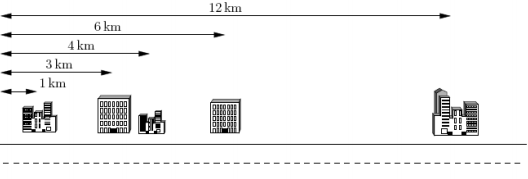
\includegraphics[width=0.9\textwidth]{bzoj1150.png}
    \end{figure}

    上例中最好的配对方案是将第 1 个和第 2 个办公楼相连,第 3 个和第 4 个办公楼相连。
    这样可按要求使用K=2 条电缆。
    第 1 条电缆的长度是 3km-1km=2km ,
    第 2 条电缆的长度是 6km-4km=2km。
    这种配对方案需要总长4km 的网络电缆,满足距离之和最小的要求。

\end{frame}

\begin{frame}{BZOJ 1150 数据备份}
    
    计算出相邻两个公司之间的距离,记为$A_i$。
    问题转化为选择序列中$K$个不相邻元素使得和最小。
    不妨用小根堆维护$A_i$。
    如果只选择一个,一定是最小的$A_i$。
    但是随选择数量的增加,可能不再选择$A_i$,
    而是选择$A_{i-1}$和$A_{i+1}$。
    且如果放弃$A_i$时一定是选择$A_{i-1}$和$A_{i+1}$,
    否则可以用$A_i$代替选中的某一元素使答案更小。
    故在选择$A_i$时,从堆中删去$A_{i-1}$和$A_{i+1}$,
    并将$\{A_{i-1},A_{i+1}\}$作为新的方案加入堆中,
    权值为$A_{i-1}+A{i+1}-A_i$。
    不断选取堆中最小值。

\end{frame}

\subsection{Binary Search}

\begin{frame}{二分 Binary Search}

    对于单调的函数,可以通过多次询问$f(x_i)$快速找到$x_t$使得$f(x_t)=y$。
    如果满足要求的$x$不唯一,还可以找到最小/大的满足要求的$x$。

    许多问题可以抽象出关于询问对象的01函数,这个函数往往具有单调性,
    如当询问对象$\geq Answer$时问题可行,当对象$< Answer$时不可行。
    求$f(x_i)$的过程就是判断对于$x_i$是否可行。

    先验证问题满足二分性质,切勿盲目二分。

    (三分适用于处理单峰函数)
    
\end{frame}

\begin{frame}{BZOJ 2525 Dynamite}

    Byteotian Cave的结构是一棵N个节点的树,其中某些点上面已经安置了bomb,现在需要点燃M个点上的引线引爆所有的bomb。
 
    某个点上的引线被点燃后的1单位时间内,在树上和它相邻的点的引线会被点燃。如果一个有bomb的点的引信被点燃,那么这个点上的bomb会爆炸。

    求引爆所有bomb的最短时间。

    $1\leq n,m \leq 300000$

\end{frame}

\begin{frame}{BZOJ 2525 Dynamite}

    二分答案,问题转化为判断能否选择$M$个点用$mid$长度覆盖全树。

    在树上自底向上贪心地选取引燃的点。

    每个子树$i$只需要记录两种状态——

    \begin{enumerate}
        \item 子树内有到$i$距离最近为$f_i$的选择点。
        \item 子树内有到$i$距离最远为$g_i$的未覆盖点。
    \end{enumerate}

    子树$i$不会同时取得$f_i$和$g_i$,
    因为如果对应的选择点可以覆盖未覆盖点,则没有未覆盖点,
    如果对应的选择点不能覆盖未覆盖点,则只上报$g_i$即可,
    外面选取的用来覆盖该为覆盖点的选择点可以覆盖$f_i$对应选择点能覆盖的点。

\end{frame}

\begin{frame}{BZOJ 4552 排序}

    在2016年,佳媛姐姐喜欢上了数字序列。

    因而她经常研究关于序列的一些奇奇怪怪的问题,现在他在研究一个难题,需要你来帮助他。

    这个难题是这样子的:给出一个1到n的全排列,现在对这个全排列序列进行m次局部排序,排序分为两种:

    \begin{enumerate}
        \item (0,l,r)表示将区间[l,r]的数字升序排序
        \item (1,l,r)表示将区间[l,r]的数字降序排序
    \end{enumerate}

    最后询问第q位置上的数字。

    $1 \leq n,m \leq 10^5$

\end{frame}

\begin{frame}{BZOJ 4552 排序}

    二分答案,把大于等于mid的数字赋值为1,把小于mid的数字赋值为0。

    每次排序相当于取一个区间内的0和1,然后

    \begin{enumerate}
        \item 如果升序排序,把0靠左放,把1靠右放。
        \item 如果降序排序,把1靠左放,把0靠右放。
    \end{enumerate}
    
    用线段树区间求和、区间赋值支持。

    最终如果第q位置为0,则mid偏大,如果第q位置为1,则mid偏小。
    
\end{frame}

\begin{frame}{BZOJ 2527 Meteors}

    有n个国家和m个空间站,每个空间站都属于一个国家,
    一个国家可以有多个空间站,所有空间站按照顺序形成一个环,
    也就是说,m号空间站和1号空间站相邻。
    现在,将会有k场流星雨降临,
    每一场流星雨都会给区间[li,ri]内的每个空间站带来ai单位的陨石,
    每个国家都有一个收集陨石的目标pi,即第i个国家需要收集pi单位的陨石。 
    
    询问:每个国家最早完成陨石收集目标是在第几场流星雨后,如果所有流星雨结束后某个国家还未完成收集目标则输出NIE。

    $1\leq n \leq m \leq 300000$

\end{frame}

\begin{frame}{CodeForces 732D}

    一共要考m场试。
    
    给出一串数字,代表了第i天能够进行哪场考试,如果为0就不能考试,每天只能考一场。
    
    一个序列a[i],每门科目要a[i]的复习时间,即需要在考试前留出a[i]天复习该科目。
    
    问最快第几天能够考完所有科目。
    
\end{frame}

\begin{frame}{CodeForces 732D}

    二分答案,判断能否在mid天内考完所有科目。

    将每个科目的考试都安排在第mid天前最靠后的时间,
    正向扫描一遍,维护当前有多少天空闲可以用于复习,
    遇到一个考试就减去其需要的复习天数,小于0则不可行。
    
\end{frame}

\begin{frame}{HDU 6241 Color a Tree}

    给定大小为N的树,初始点都是白色。

    请你染色以满足a+b个限制,求最少染色点数。

    a个限制1,形如(1, X, Y),表示X子树至少有Y个点被染色。

    b个限制2,形如(2, X, Y),表示X子树外至少有Y个点被染色。

\end{frame}

\begin{frame}{HDU 6241 Color a Tree}

    答案满足二分性质(最差把所有点都染色)。

    要通过染色不多于mid个点满足限制,可以将两种限制归一如下——

    \begin{enumerate}
        \item (1, X, Y) X子树内至少Y个点被染色
        \item (2, X, Y) X子树内最多mid-Y个点被染色
    \end{enumerate}

    自底向上push一遍检查是否可行。
    
\end{frame}

\begin{frame}{BZOJ 2527 Meteors}
    
    整体二分。

    如果只询问第$i$个国家的答案,可以二分完成——将前mid次流星雨加入,查询第$i$个国家的所有空间站陨石之和。

    要对每个国家都回答问题,可以让它们一起二分。

    \begin{enumerate}
        \item 为每个国家初始化二分区间为$[0,\infty]$并计算mid
        \item 将所有国家按照mid从小到大排序
        \item 在树状数组/线段树中依次加入前$i$场流星雨,如果$i=mid_j$,则查询国家$j$的所有空间站陨石之和$res_j$
        \item 根据每个国家查询到的$res_j$判断mid偏大偏小,并产生新的二分区间
        \item 如果所有国家二分区间都缩为一个点,停止;否则从第2步再来一遍
    \end{enumerate}

\end{frame}

\begin{frame}{BZOJ 2738 矩阵乘法}

    给你一个$N\times N$的矩阵,每次询问一个子矩形的第K小数。
    
    N,Q分别表示矩阵大小和询问组数;
    
    $N\leq 500,Q\leq 60000。$
    
\end{frame}

\begin{frame}{BZOJ 2738 矩阵乘法}
    
    整体二分。
    
    \begin{enumerate}
        \item 将矩阵所有元素从小到大排序
        \item 为每个询问初始化二分区间为$[-\infty,+\infty]$并计算mid
        \item 将所有询问按照mid从小到大排序
        \item 在二维树状数组依次加入前$i$个元素,如果$i=mid_j$,则查询询问$j$子矩形内此时元素个数
        \item 根据查询结果产生新的二分区间
        \item 如果所有询问二分区间缩为一点,停止;否则从第3步再来一遍
    \end{enumerate}
    
\end{frame}

\subsection{Divide and Conquer}

\begin{frame}{分治 Divide and Conquer}

    \begin{itemize}
        \item 序列分治
        \item CDQ分治
        \item 点分治
        \item 边分治
        \item 动态点分治
        \item 动态边分治
        \item ……
    \end{itemize}
    
\end{frame}

\begin{frame}{BZOJ 2287 消失之物}

    ftiasch 有$N$个物品, 体积分别是$W_1,W_2,...,W_N$。 
    由于她的疏忽, 第$i$个物品丢失了。 
    “要使用剩下的$N-1$物品装满容积为$x$的背包,有几种方法呢?” 
    这是经典的问题了,她把答案记为$Count(i, x)$。
    想要得到所有$1\leq i \leq N, 1 \leq x \leq M$的$Count(i,x)$表格。

    $1\leq N\leq 2\times 10^3$

    $1\leq M\leq 2\times 10^3$

\end{frame}

\begin{frame}{BZOJ 2287 消失之物}

    将区间$[1,N]$等分为两个小区间$[1,mid],[mid+1,N]$。

    删去左边区间内物品时,右边区间内物品都可以加入背包;

    删去右边区间内物品时,左边区间内物品都可以加入背包。

    每层将右边物品加入背包,递归进入左区间;
    回溯之后恢复状态,加入左区间物品后递归进入右区间。

    每层加入$O(N)$个物品,一共$O(logN)$层。
    
\end{frame}

\begin{frame}{POJ 3233 Matrix Power Series}
    
    Given a n × n matrix A and a positive integer k, find the sum $S = A + A^2 + A^3 + \ldots +A^k.$
    
    Output the elements of S modulo m in the same way as A is given.
    
    $n \leq 30$
    
    $k \leq 10^9$
    
    $m \leq 10^4$

\end{frame}

\begin{frame}{POJ 3233 Matrix Power Series}

    如果k为偶数,则
    $$sum(k) = (1+A^{\frac{k}{2}}) ( A+A^2+\ldots+A^{\frac{k}{2}}) = (1+A^{\frac{k}{2}})  sum(\frac{k}{2})$$
    
    如果k为奇数,则
    $$sum(k) = sum(k-1) + A^k$$

    递归即可,需要矩阵快速幂的支持。

    有人将这种思想称为奇偶分治。

\end{frame}

\begin{frame}{POJ 3233 Matrix Power Series}

    其实可以构造一个$2n \times 2n$的矩阵
    $$
    B = \begin{bmatrix}
        E_n & 0 \\
        A & E_n \\
    \end{bmatrix}
    $$
    则求
    $$
    B^k \begin{bmatrix}
        A \\
        0 \\
    \end{bmatrix}
    $$
    一次矩阵快速幂即可。

\end{frame}

\begin{frame}{BZOJ 3697 采药人的路径}

    采药人的药田是一个树状结构,每条路径上都种植着同种药材。

    采药人以自己对药材独到的见解,对每种药材进行了分类。大致分为两类,一种是阴性的,一种是阳性的。

    采药人每天都要进行采药活动。他选择的路径是很有讲究的,他认为阴阳平衡是很重要的,所以他走的一定是两种药材数目相等的路径。
    
    采药工作是很辛苦的,所以他希望他选出的路径中有一个可以作为休息站的节点(不包括起点和终点),满足起点到休息站和休息站到终点的路径也是阴阳平衡的。
    
    他想知道他一共可以选择多少种不同的路径。

    $N\leq 10^5$

\end{frame}

\begin{frame}{BZOJ 3697 采药人的路径}
    
    点分治。

    如果没有休息站的限制,那么统计分治子树内到分治根结点的所有竖直路径阴阳差值即可。

    要满足休息站要求,需要将路径分为
    
    \begin{enumerate}
        \item 包含至少一个阴阳平衡点的路径
        \item 不包含阴阳平衡点
    \end{enumerate}

    还是在分治根结点计算经过分治根结点的答案。

\end{frame}

\begin{frame}{BZOJ 3648 寝室管理}

    T128的寝室条件不是很好,所以没有很多钱来装修。
    寝室仅由n-1条双向道路连接,而且任意两间寝室之间都可以互达。
    最近,T128被要求对一条路径上的所有寝室进行管理,这条路径不会重复经过某个点或某条边。
    但他不记得是哪条路径了,他只记得这条路径上有不少于k个寝室。
    于是,他想请T64帮忙数一下,有多少条这样的路径满足条件。 
    
    还有一个问题。
    由于最近有一些熊孩子不准晚上讲话很不爽,
    他们决定修筑一条“情报通道”。
    如果通道建成,寝室就变成了一个N个点N条边的无向图。
    并且,经过“情报通道”的路径也是合法的。
    T128心想:通道建成之前,T64还有一个高效的算法帮我数路径条数,
    但是通道建成之后,他还有办法吗?
    对,T64手忙脚乱,根本数不清有多少条路径。于是他找到了你。

    $n\leq 10^5$

\end{frame}

\begin{frame}{BZOJ 3648 寝室管理}

    如果没有情报通道,那么构成一棵树,可以通过点分治计算答案。

    如果加入情报通道,变成了基环树。
    首先用点分治计算不经过环的子树内答案。
    然后统计子树内到环上点的距离,
    在环上计算经过环的答案。

    提示:可以将环断开成链并加倍以方便处理。

\end{frame}

\begin{frame}{BZOJ 1176 Mokia}

    有一个$n \times n$的棋盘,每个格子内有一个数,初始的时候全部为0.现在要求维护两种操作:

    \begin{enumerate}
        \item Add: 将格子$(x,y)$内的数加上$z$
        \item Query: 求矩阵$(x0, y0, x1, y1)$内所有数字之和
    \end{enumerate}

    Add $\leq 160000$
    
    Query $\leq 10000$
    
    $n \leq 2000000$
    
\end{frame}

\begin{frame}{BZOJ 1176 Mokia}
    
    CDQ分治 
    
    按照时间维度分治,计算左区间内操作对右区间内询问的影响。

    \begin{itemize}
        \item 操作和询问一起按照时间维度排序
        \item 左区间内的Add对右区间的Query有影响,用扫描线+树状数组计算
        \item 递归左区间、右区间
    \end{itemize}
    
\end{frame}

\begin{frame}{BZOJ 3262 陌上花开}
    
    有n朵花,每朵花有三个属性:花形(s)、颜色(c)、气味(m),用三个整数表示。
    现要对每朵花评级,一朵花的级别是它拥有的美丽能超过的花的数量。
    定义一朵花A比另一朵花B要美丽,
    当且仅当$S_a \geq S_b,C_a \geq C_b,M_a\geq M_b$。
    显然,两朵花可能有同样的属性。
    需要统计出评出每个等级的花的数量。

    $N$,$K$分别表示花的数量和最大属性值。

    $1 \leq N \leq 100000, 1 \leq K \leq 200000$

\end{frame}

\begin{frame}{BZOJ 3262 陌上花开}
    
    三维偏序。

    CDQ分治解决一维,排序解决一维,树状数组解决一维。

\end{frame}

\subsection{Multiplication}

\begin{frame}{倍增 Multiplication}

    \begin{itemize}
        \item 快速幂
        \item 矩阵快速幂
        \item ST表
        \item LCA
        \item 奇妙应用
    \end{itemize}
    
\end{frame}

\begin{frame}{BZOJ 1297 迷路}

    有N个点,若干条带长度的边。

    询问长度为K的从1到N的路径数量。

    $N\leq 10$
    $D_i\leq 9$
    
\end{frame}

\begin{frame}{BZOJ 1297 迷路}

    如果边权相同,计算邻接矩阵的K次幂即可。

    边权不同但是注意到边权不会大于9。

    原先的每个点$i$拆为新的9个点
    $(i,1),(i,2)\ldots(i,9)$,
    且在$(i,t)$和$(i,t+1)$之间连边。

    如果$i$和$j$之间有长度为$d$的边,
    则在新图中连边$(i,d)$和$(i,1)$。
    
\end{frame}

\begin{frame}{HDU 6395 Sequence}

    Let us define a sequence as below

    $f(n) = d f(n-1) + c f(n-2) + \lfloor\frac{p}{n}\rfloor$

    $f(1)=a, f(2)=b$

    $1 \leq T \leq 20, 0 \leq a, b, c, d, p, n \leq 10^9$

    Your job is simple, for each task, you should output $f(n)$ module $10^9+7$.

\end{frame}

\begin{frame}{HDU 6395 Sequence}

    注意到对于一个$p$和不同的$n$,$\lfloor\frac{p}{n}\rfloor$只有$O(\sqrt{p})$种不同的取值。

    分为$O(\sqrt{p})$段,每一段内转移矩阵相同,用矩阵快速幂计算。
    
\end{frame}

\begin{frame}{HDU 4291 A Short Problem}

    Given $n$ ($1\leq n\leq 10^{18}$),
    you should solve for g(g(g(n))) mod $10^9+7$.

    $g(n) = 3g(n–1) + g(n–2)$
    
    $g(1) = 1$
    
    $g(0) = 0$

\end{frame}

\begin{frame}{HDU 4291 A Short Problem}

    如果是计算g(n) mod P,矩阵快速幂即可。

    但是g(g(n)) mod P$\not =$g(g(n mod P)) mod P。

    大胆猜测g(n) mod P有循环节,暴力求出循环节长度记为$P_1$。

    同理求出g(n) mod $P_1$的循环节长度记为$P_2$。

    计算g(g(g(n) mod $P_2$) mod $P_1$) mod P即可。

    三次矩阵快速幂,在不同的模数下。
    
\end{frame}

\begin{frame}{POJ 2452 Sticks Problem}

    Xuanxuan has n sticks of different length. One day, she puts all her sticks in a line, represented by S1, S2, S3, ...Sn. After measuring the length of each stick Sk (1 <= k <= n), she finds that for some sticks Si and Sj (1<= i < j <= n), each stick placed between Si and Sj is longer than Si but shorter than Sj. 

    Now given the length of S1, S2, S3, …Sn, you are required to find the maximum value j - i.

    $n \leq 50000$

\end{frame}

\begin{frame}{POJ 2452 Sticks Problem}

    枚举$i$,通过二分查找求$i$右边最远的$j$使得$S_i=min(S_i,...,S_j)$,
    再找到$k=argmax(S_i,...,S_j)$,$[i,k]$即为左端点为$i$时的最优解。

\end{frame}

\begin{frame}{POJ 2019 Cornfields}
    
    FJ has decided to grow his own corn hybrid in order to help the cows make the best possible milk. To that end, he's looking to build the cornfield on the flattest piece of land he can find. 

    FJ has, at great expense, surveyed his square farm of N x N hectares (1 <= N <= 250). Each hectare has an integer elevation (0 <= elevation <= 250) associated with it. 

    FJ will present your program with the elevations and a set of K (1 <= K <= 100,000) queries of the form "in this B x B submatrix, what is the maximum and minimum elevation?". The integer B (1 <= B <= N) is the size of one edge of the square cornfield and is a constant for every inquiry. Help FJ find the best place to put his cornfield. 

\end{frame}

\begin{frame}{POJ 2019 Cornfields}
    
    二维线段树模板题,但也可以用二维ST表。

    $F[x][y][i][j]$为以$(x,y)$为左上角,长$2^i$,宽$2^j$的子矩形内最大值。

    $G[x][y][i][j]$为以$(x,y)$为左上角,长$2^i$,宽$2^j$的子矩形内最小值。

    每一个询问的子矩形可以拆分为四个可能重叠的子矩形。

\end{frame}

\begin{frame}{BZOJ 4569 萌萌哒}

    一个长度为n的大数,用$S_1S_2S_3\ldots Sn$表示,
    其中$S_i$表示数的第i位,$S_1$是数的最高位。
    告诉你一些限制条件,每个条件表示为四个数,
    $l_1,r_1,l_2,r_2$,
    即两个长度相同的区间,
    表示子串$S_{l1}S_{l1+1}S_{l1+2}...S_{r1}$与$S_{l2}S_{l2+1}S_{l2+2}...S_{r2}$完全相同。
    
    比如n=6时,某限制条件l1=1,r1=3,l2=4,r2=6,那么123123,351351均满足条件,但是12012,131141不满足条件,前者数的长度不为6,后者第二位与第五位不同。
    
    问满足以上所有条件的数有多少个。
    
    n和m,分别表示大数的长度,以及限制条件的个数。
    
    $1 \leq n \leq 10^5,1 \leq m \leq 10^5$

\end{frame}

\begin{frame}{BZOJ 4569 萌萌哒}

    通过限制条件找出所有集合,集合内元素相同。
    包含$S_1$的集合取值有9种,其它集合取值有10种。
    记集合个数为$k$,则答案为$9\times 10^{k-1}$。

    朴素并查集无法维护合并集合的操作,考虑用ST表的思想优化。

    建立一些结点,$(i,j)$对应$[i,i+2^j-1]$区间。
    用这些结点构成并查集的结点。
    如果要合并两个区间,首先将每个区间拆分为最大的两个重叠区间,得到的四个区间也是两两对应的。
    将对应结点合并,如果已经连通则退出,否则还要尝试递归合并更小的区间。

    注意到总的结点个数为$O(NlogN)$。

\end{frame}

\begin{frame}{BZOJ 3251 树上三角形}

    给定一大小为n的有点权树。
    
    每次询问一对点(u,v),问是否能在u到v的简单路径上取三个点权,
    以这三个权值为边长构成一个三角形。
    
    同时还要求支持单点修改。
    
\end{frame}

\begin{frame}{BZOJ 3251 树上三角形}

    考虑路径上的数字从小到大排列,
    如果其中元素不能构成三角形,
    则有$a_i\geq a_{i-1} + a_{i-2}$,
    故这个序列增长速度不慢于斐波那契数列。

    众所周知,斐波那契数列指数级增长,所以上面的序列$a_i$很快超过int。

    可以知道,路径长度大于50时,一定不满足上面的不等式,即一定有解。
    
    路径长度不超过50暴力即可。

    倍增是用来求LCA的。
    
\end{frame}

\begin{frame}{BZOJ 4082 Surveillance}

    The International Corporation for Protection and Control (ICPC) develops efficient technology for,well, protection and control. Naturally, they are keen to have their own headquarters protected and controlled. Viewed from above, the headquarters building has the shape of a convex polygon. There are several suitable places around it where cameras can be installed to monitor the building. Each camera covers a certain range of the polygon sides (building walls), depending on its position. ICPC wants to minimize the number of cameras needed to cover the whole building.

    n个点的环和k个区间,用最少的区间覆盖整个环。

    $3 \leq n \leq 10^6$

    $1 \leq k \leq 10^6$

\end{frame}

\begin{frame}{BZOJ 4082 Surveillance}
    
    n个点构成线段的情况是基本功,贪心寻找能跳到的最远点即可。

    对于环的情形,枚举从哪个区间出发,按照同样的贪心策略,跳尽可能少的步数覆盖整个环,用倍增优化这个过程。

    记$f_{i,0}$为区间i能跳到的右端点最靠右的区间, \\
    $f_{i,1}$为区间i出发跳两次能跳到的最靠右的区间, \\
    $f_{i,j}$为区间i出发跳$2^j$能跳到的最靠右的区间。

\end{frame}

\section{Exercises}

\subsection{Kick Start}

\begin{frame}{Google Kick Start}

    \begin{itemize}
        \item g.co/kickstart
        \item Google校园招聘的敲门砖
        \item 个人赛,3道题3小时,题目难度飘忽不定
        \item 获得全球TOP100可能会获得各种活动邀请
        \item \sout{然鹅成绩大约2年有效,现在打排名并木有用}
    \end{itemize}
    
\end{frame}

\begin{frame}{Round A 2019 Training}

    As the football coach at your local school, you have been tasked with picking a team of exactly P students to represent your school. There are N students for you to pick from. The i-th student has a skill rating Si, which is a positive integer indicating how skilled they are.

    You have decided that a team is fair if it has exactly P students on it and they all have the same skill rating. That way, everyone plays as a team. Initially, it might not be possible to pick a fair team, so you will give some of the students one-on-one coaching. It takes one hour of coaching to increase the skill rating of any student by 1.
    
    The competition season is starting very soon (in fact, the first match has already started!), so you'd like to find the minimum number of hours of coaching you need to give before you are able to pick a fair team.
    
    Time limit: 15 seconds per test set. Memory limit: 1 GB.\\
    $1\leq T\leq 100, 1\leq S_i\leq 10000, 2\leq P\leq N$\\
    Test set 1 (Visible) $2\leq N\leq 1000$\\
    Test set 2 (Hidden) $2\leq N\leq 10^5$
    
\end{frame}

\begin{frame}{Round A 2019 Training}

    首先对所有学生按照技能值从小到大排序,
    显然选中的代表队应当为其中连续的一段,
    应当通过训练使该区间内所有学生的技能值达到区间内最大技能值。
    
    从左向右枚举长度为$P$的区间,则选取$[l,r]$区间所需最少训练时间为
    $cost_{l,r}=\sum_{i=l}^{r}{|S_i-S_r|}$。
    预先计算前缀和即可快速查询区间和,或者在区间移动时维护变化量亦可。
    由此可以在$O(1)$时间内求得$cost_{l,r}$。
    
    时间复杂度$O(NlogN)$
    
    空间复杂度$O(N)$
    
\end{frame}

\begin{frame}{Round A 2019 Parcels}

    You have been hired recently as the Chief Decision Maker (CDM) at a famous parcel delivery company, congratulations! Customers love speedy deliveries of their parcels and you have decided to decrease the time it takes to deliver parcels around the world to win customers. You have introduced this idea to the authorities and they have allocated you enough budget to build at most one new delivery office.

    The world can be divided into an R × C grid of squares. Each square either contains a delivery office or it does not. You may pick a grid square that does not already contain a delivery office and build a new delivery office there.
    
    The delivery time of a parcel to a square is 0 if that square contains a delivery office. Otherwise, it is defined as the minimum Manhattan distance between that square and any other square containing a delivery office. The overall delivery time is the maximum of delivery times of all the squares. What is the minimum overall delivery time you can obtain by building at most one new delivery office?
    
\end{frame}

\begin{frame}{Round A 2019 Parcels}
    
    Note: The Manhattan distance between two squares (r1,c1) and (r2,c2) is defined as |r1 - r2| + |c1 - c2|, where |*| operator denotes the absolute value.
    
    Time limit: 15 seconds per test set. Memory limit: 1GB. \\
    $1 \leq T \leq 100$ There is at least one delivery office in the initial grid. \\
    Test set 1 (Visible) $1\leq R\leq 10, 1\leq C\leq 10$\\
    Test set 2 (Hidden) $1\leq R\leq 250, 1\leq C\leq 250$
    
\end{frame}

\begin{frame}{Round A 2019 Parcels}

    显然答案满足二分性质。
    应用二分之后问题转化为对于一个给定的$K$,
    能否在某一方格建立新的快递点,
    使得之后任何方格到最近有快递点方格的曼哈顿距离不超过$K$。
    
    不难看出,到一个点$(x,y)$曼哈顿距离不超过$K$的方格
    组成一个旋转$45^{\circ}$的正方形,不妨记为$<(x,y),K>$。
    可以先考虑哪些方格在当前已经有的快递点状态下就满足要求,
    这些点可以通过BFS在$O(RC)$时间内求出。
    而后对于一个当前不满足要求的点$(x_i,y_i)$,必须在$<(x_i,y_i),K>$内安置快递点。
    要判断是否存在解,只需要对所有正方形求交集,看是否为空集。
    
    两个矩形可以非常简单地求交集,
    且交集一定也是一个矩形。
    对至多$RC$个正方形求交时间复杂度为$O(RC)$。
    
    时间复杂度$O(RClog_2{RC})$
    
    空间复杂度$O(RC)$
    
\end{frame}

\begin{frame}{Round C 2019 Circuit Board}

    Arsh recently found an old rectangular circuit board that he would like to recycle. The circuit board has R rows and C columns of squares.

    Each square of the circuit board has a thickness, measured in millimetres. The square in the r-th row and c-th column has thickness Vr,c. A circuit board is good if in each row, the difference between the thickest square and the least thick square is no greater than K.
    
    Since the original circuit board might not be good, Arsh would like to find a good subcircuit board. A subcircuit board can be obtained by choosing an axis-aligned subrectangle from the original board and taking the squares in that subrectangle. Arsh would like your help in finding the number of squares in the largest good subrectangle of his original board.
    
    Time limit: 15 seconds per test set. Memory limit: 1GB.\\
    $1\leq T\leq 50, 1\leq R\leq 300, 1\leq C\leq 300, 0\leq V_{i,j}\leq 10^3$\\
    Test set 1 (Visible) $K=0$
    Test set 2 (Hidden) $0\leq K\leq 10^3$
    
\end{frame}

\begin{frame}{Round C 2019 Circuit Board}

    行与行之间无关。
    
    枚举$i,j$,表示选择第$i$行到第$j$行。
    
    预处理每个点作为右端点时的最小左端点。
    
    在枚举$i,j$同时对预处理做前缀和处理。
    
    时间复杂度 $O(RClogC)$
    
\end{frame}

\begin{frame}{Round C 2019 Catch Some}

    Bundle is an animal researcher and needs to go observe K dogs. She lives on a horizontal street marked at metre increments with consecutive numbers 0, 1, 2, 3 and so on. She begins in her home, which is at position 0. There are also N dogs on the street. The i-th dog is Pi metres to the right of her home on the street (multiple dogs can share the same position).
    
    Dogs come in different colors, which are denoted by positive integers. The i-th animal is of color Ai.
    
    If Bundle is at her home, she can change the current color of her shirt. This is important since the dogs are very shy! Bundle can only observe a dog if she is at the same position as that dog, and is wearing a shirt of the same color as the dog.
    
    It takes Bundle one second to move one metre to the left or right on the street. It takes her no time to change shirts or observe a dog.
    
    What is the least amount of time it will take Bundle to observe K dogs? Note that she does not have to return home after observing K dogs.
    
\end{frame}

\begin{frame}{Round C 2019 Catch Some}

    Time limit: 30 seconds per test set. Memory limit: 1GB.\\
    $1\leq T\leq 100, 1\leq K\leq N, 1\leq A_i\leq 1000, 1\leq P_i\leq 10^5$\\
    Test set 1 (Visible) $1\leq N\leq 50$\\
    Test set 2 (Hidden) $1\leq N\leq 1000$
    
\end{frame}

\begin{frame}{Round C 2019 Catch Some}

    分类01背包问题的变种。
    
    对于一种颜色,可能有若干只狗狗分布在数轴上,主人公如果和其中$k$只互动,一定是从家出发,依次和坐标最小的前$k$只互动,然后可能返回家也可能不返回,取决于是否是互动的最后一只狗狗。如果设这种颜色的狗狗的坐标从小到大排序后为序列$A_i$,那么和$k$只狗狗互动的最小代价是$2\times A_k$或$A_k$,取决于是否返回。
    
    先不考虑最后一次互动后不用返回。对于每种颜色,我们需要确定一个$k$,代表和$k$只这种颜色的狗狗互动。要求所有的$k$的和应当为$K$,同时我们希望最小化$2 \times A_k$的和。这就是分类01背包问题。
    
    因为最后一次互动后不需返回,那么有一类代价可以计为$A_k$而非$2\times A_k$。设$F_{i,j}$表示在前$i$个分类中,一共取了$j$个物品,每个物品的代价都是按$2\times A_k$计的最小代价;$G_{i,j}$表示在前$i$个分类中,一共取了$j$个物品,有一个物品代价按$A_k$计的最小代价。做类似的DP即可,$G$数组的求解依赖于$F$数组。
    
\end{frame}

\begin{frame}{Round A 2019 Contention}

    You are selling tickets for the front row of seats at a movie theater. The front row has N seats, numbered 1 to N from left to right. You have been out of the office the last week, and upon your return, Q bookings for seats have piled up! The i-th booking requests all the seats from Li to Ri inclusive. You now have the boring job of entering each booking into the system, one at a time.

    Since some of the bookings may overlap, the system might not be able to fulfill each booking entirely. When you enter a booking into the system, it will assign every seat requested by the booking that hasn't already been assigned to a booking entered into the system earlier.
    
    What is the largest integer k where there exists an order that you can enter the bookings into the system, such that each booking is assigned at least k seats?
    
    Time limit: 30 seconds per test set. Memory limit: 1GB.\\
    $T=100,1\leq N\leq 10^6,1\leq L_i\leq R_i\leq N$\\
    Test set 1 (Visible) $1\leq Q\leq 300$\\
    Test set 2 (Hidden) $1\leq Q\leq 30000$\\
    For at least 85 of the test cases, $Q\leq 3000$

\end{frame}

\begin{frame}{Round A 2019 Contention}

    考虑从$Q$个订购请求中选取一个放在最后的位置,那么这个请求所获的的座位数和之前$Q-1$个请求的顺序无关。可以计算出每一个请求放在最后所能获得座位数,选取最大者固定在最后,再将另外$Q-1$个请求递归解决。可以证明,这样的贪心算法是正确的(可以考虑交换倒数第一和倒数第二,结果不会变优,而任何其他排列可以通过若干次这样的交换达到,故贪心策略正确)。

    要维护贪心过程,需要用线段树维护每个座位在当前多少个请求中。需要支持区间加法和减法。当一个座位只属于一个请求时,我们就可以把该座位分配给这个请求。当一个座位被购买后,在线段树中将该点的值修改为正无穷,以防之后在求区间最小值的过程中影响算法。还需要支持查询一个只属于一个请求的座位,究竟属于哪个请求。方法是在线段树上每个节点开一个set,记录恰好覆盖该结点的请求。从一个叶子结点出发向上爬,遇到的第一个非空set中的元素就是包含该座位的区间。
    
    可以预先将座位分段,化$O(N)$为$O(Q)$。
    
    时间复杂度$O(QlogQ)$
    
    空间复杂度$O(Q)$
    
\end{frame}

\begin{frame}{BZOJ 3728 Final Zarowki}

    有n个房间和n盏灯,你需要在每个房间里放入一盏灯。每盏灯都有一定功率,每间房间都需要不少于一定功率的灯泡才可以完全照亮。 
    你可以去附近的商店换新灯泡,商店里所有正整数功率的灯泡都有售。但由于背包空间有限,你至多只能换k个灯泡。 
    你需要找到一个合理的方案使得每个房间都被完全照亮,并在这个前提下使得总功率尽可能小。
    (初始n盏灯的功率为序列$p_i$,输入给定)

    $1 \leq k \leq n \leq 500000$
    
\end{frame}

\begin{frame}{BZOJ 3728 Final Zarowki}

    将所有房间按照需要功率从大到小排序,
    依次枚举每一个房间,
    将能照亮此房间的灯加入最小堆,
    取出功率最小的能照亮此房间的灯分配给这个房间。
    如果堆为空,则从商店换一个最小功率的灯来照亮这个房间。
    如果堆为空且已经没有剩余换灯泡机会,则无解。
    最终可能剩余若干次换灯泡机会,用在灯泡功率-需求功率最大的若干者上。
    
\end{frame}

\begin{frame}{BZOJ 1029 建筑抢修}

    小刚在玩JSOI提供的一个称之为“建筑抢修”的电脑游戏:
    经过了一场激烈的战斗,T部落消灭了所有z部落的入侵者。
    但是T部落的基地里已经有N个建筑设施受到了严重的损伤,
    如果不尽快修复的话,这些建筑设施将会完全毁坏。
    现在的情况是:T部落基地里只有一个修理工人,
    虽然他能瞬间到达任何一个建筑,但是修复每个建筑都需要一定的时间。
    同时,修理工人修理完一个建筑才能修理下一个建筑,不能同时修理多个建筑。
    如果某个建筑在一段时间之内没有完全修理完毕,这个建筑就报废了。
    你的任务是帮小刚合理的制订一个修理顺序,以抢修尽可能多的建筑。

    $N\leq 150000$
    
\end{frame}

\begin{frame}{BZOJ 1029 建筑抢修}

    记$A_i$为抢修$i$需要时间,$B_i$为维修$i$时间限制。

    直观想法是按照$B_i$排序,
    从小到大枚举$i$,能修复则修复,否则就跳过。

    显然是有漏洞的,比如 (10, 10), (10, 20), (2, 21), (2, 21)。

    完善策略,如果当前枚举到$i$时发现空闲时间不足修复该建筑,
    但是之前维修的$j$满足$A_j < A_i$,则用维修$i$而放弃$j$,
    这样当前答案没有减少但是空闲时间多了,对后续决策有利。
    
\end{frame}


\end{document}
